% Gemini theme
% https://github.com/anishathalye/gemini

\documentclass[final]{beamer}

% ====================
% Packages
% ====================

\usepackage[T1]{fontenc}
\usepackage{lmodern}
\usepackage[size=custom,width=91.44,height=121.92,scale=1.25]{beamerposter}
\usetheme{gemini}
\usecolortheme{gemini}
\usepackage{graphicx}
\usepackage{booktabs}
\usepackage{tikz}
\usepackage{pgfplots}
\pgfplotsset{compat=1.14}
\usepackage{anyfontsize}

% ====================
% Flowchart Style
% ====================

\tikzstyle{startstop} = [rectangle, minimum width=3cm, minimum height=1cm, text
centered, draw=black, fill=red!30]

\tikzstyle{io} = [rectangle, minimum width=3cm, minimum height=1cm, text
centered, draw=black, fill=blue!30]

\tikzstyle{process} = [rectangle, minimum width=3cm, minimum height=1cm, text
centered, draw=black, fill=orange!30]

\tikzstyle{decision} = [rectangle, minimum width=3cm, minimum height=1cm, text
centered, draw=black, fill=green!30]

\tikzstyle{arrow} = [thick,->,>=stealth]

% ====================
% Lengths
% ====================

% If you have N columns, choose \sepwidth and \colwidth such that
% (N+1)*\sepwidth + N*\colwidth = \paperwidth
\newlength{\sepwidth}
\newlength{\colwidth}
\setlength{\sepwidth}{0.02\paperwidth}
\setlength{\colwidth}{0.47\paperwidth}

\newcommand{\separatorcolumn}{\begin{column}{\sepwidth}\end{column}}

  % ====================
  % Title
  % ====================

  \title{\texttt{build-pulse}: A Research-Focused Jenkins CI/CD Static Build
  Analyzer}

  \author{Ethan Wong \inst{1}\inst{2} \and Hui Zhou \inst{2}}

  \institute[shortinst]{\inst{1} University of Illinois at Chicago
  \samelineand \inst{2} Argonne National Laboratory}

  % ====================
  % Footer (optional)
  % ====================

  \footercontent{
\includegraphics[height=4cm]{doe.pdf} \hfill
  
\includegraphics[height=4cm]{anl.pdf}}
  % (can be left out to remove footer)

  % ====================
  % Logo (optional)
  % ====================

  % use this to include logos on the left and/or right side of the header:
  % \logoright{\includegraphics[height=7cm]{logo1.pdf}}
  % \logoleft{\includegraphics[height=7cm]{logo2.pdf}}

  % ====================
  % Body
  % ====================

  \begin{document}

  \begin{frame}[t]
    \begin{columns}[t]
      \separatorcolumn

      \begin{column}{\colwidth}
        \begin{alertblock}{Motivation}
          Complex software projects commonly rely upon continuous-integration
          and continuous-deployment (CI/CD) platforms to configure extensive
          build pipelines which streamline development. A single pipeline often
          holds a substantial number of jobs, each packaging and testing a
          unique configuration permutation for correctness.

          Introducing even a single regression has the ability to propagate
          failures across an entire pipeline. These regressions cause
          maintainers to waste significant time finding often trivial underlying
          issues. \texttt{build-pulse\cite{github}} mitigates the impact of
          these regressions by exhaustively analyzing build pipelines defined in
          Jenkins, a popular CI/CD platform, coalescing build failures by their
          underlying issues, and prioritizing regressions by their severity,
          eliminating manual debugging for maintainers.
        \end{alertblock}

        \begin{exampleblock}{Program Flow}
          \heading{Stages}
          \begin{enumerate}
            \item Artifacts from the runs of each job build configuration are
              pulled from the Jenkins API and cached in a database to be parsed
            \item Unparsed artifacts are pattern matched for snippets which are
              tagged and stored as issues for analysis
            \item Issues are processed for similarity, prioritized, and
              aggregated as statistics tailored to maintainers' needs
            \item A static HTML report is templated with \texttt{maud} and
              outputted for simple viewing in email, webhooks, and browsers
          \end{enumerate}

          \begin{figure}
            \centering
            \begin{tikzpicture}[node distance=3cm]
              \node(start) [startstop] {Jenkins Run Jobs};
              \node(in1) [io, below of=start] {\texttt{build-pulse} Pulls
              Artifacts From Build};
              \node (dec1) [decision, below of=in1] {Build Has Failures};
              \node (pro1a) [process, below of=dec1] {Artifacts Parsed and
              Tagged};
              \node (pro1b) [process, right of=dec1, xshift=10cm] {Not
              Analyzed};

              \node (dec2) [decision, below of=pro1a] {More Builds?};
              \node (pro2) [process, left of=dec2, xshift=-10cm] {Pull Another
              Build};
              \node(in2) [io, below of=dec2] {All Failure Artifacts Parsed};

              \node (pro3) [process, below of=in2] {Issues Grouped By
              Similarity};
              \node (pro4) [process, below of=pro3] {Statistics Computed};
              \node(stop) [startstop, below of=pro4] {\texttt{build-pulse}
              Generates Report};

              \draw [arrow] (start) -- (in1);
              \draw [arrow] (in1) -- (dec1);
              \draw [arrow] (dec1) -- node[anchor=south] {no} (pro1b);
              \draw [arrow] (dec1) -- node[anchor=west] {yes} (pro1a);
              \draw [arrow] (pro1a) -- (dec2);
              \draw [arrow] (dec2) -- node[anchor=south] {yes} (pro2);
              \draw [arrow] (pro2) |- (in1);
              \draw [arrow] (dec2) -- node[anchor=west] {no} (in2);
              \draw [arrow] (in2) -- (pro3);
              \draw [arrow] (pro3) -- (pro4);
              \draw [arrow] (pro4) -- (stop);
            \end{tikzpicture}
            \caption{Stage Diagram of \texttt{build-pulse}}
          \end{figure}

          \heading{Optimization}
          \texttt{build-pulse} is aggressively optimized to maximize performance
          and maintainer productivity.
          \begin{itemize}
            \item Written in Rust with heavy utilization of \texttt{rayon}, a
              data-parallelism crate akin to OpenMP
            \item API calls are minimized using the Jenkins Tree Query
              API\cite{jenkins}
            \item All runs and their corresponding artifacts are only retrieved
              \underline{once} and cached
          \end{itemize}
        \end{exampleblock}

        \begin{block}{Issue Tagging}
          \heading{Tagging}
          \texttt{build-pulse} identifies issues and tags them using
          \underline{regular expressions}. Tag categories represent the primary
          metric aggregated on reports. Tags are defined generically in-order to
          match issues as \textit{broadly as possible} and allow for parsing to
          work on a wide variety of tooling.
          \heading{Reports}
          Identified issues are rendered in reports with their snippet and
          corresponding run information.
          \begin{figure}
            \centering
            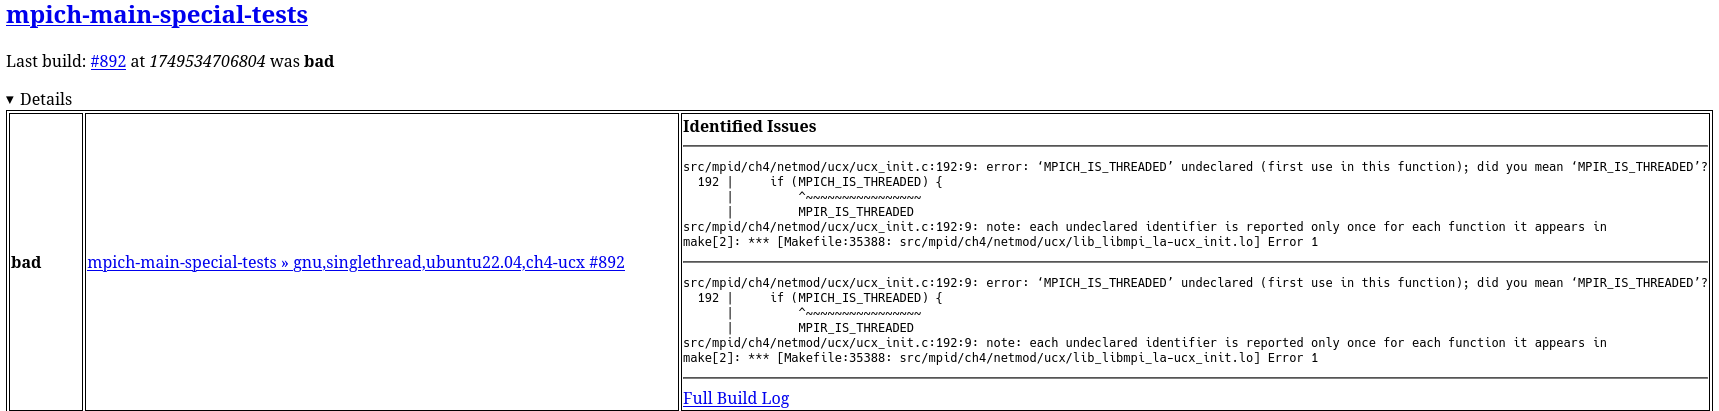
\includegraphics[width=\linewidth]{report.png}
            \caption{Example Report Showing an Identified \texttt{cc\_emit}}
          \end{figure}
        \end{block}
      \end{column}

      \separatorcolumn

      \begin{column}{\colwidth}
        \begin{block}{Defining Similarity}
          Issues are conservatively grouped and considered ``similar'' if the
          normalized Levenshtein distance of their snippets meet a fixed
          threshold.

          \heading{Recursive Definition}
          The Levenshtein distance metric\cite{levenshtein} considers the
          difference between two snippets $a, b$ as the minimum number of edits
          needed for $a \rightarrow b$.

          \begin{math}
            {\displaystyle \operatorname {lev} (a,b)={\begin{cases}|a|&{\text{
                if }}|b|=0,\\|b|&{\text{ if }}|a|=0,\\\operatorname {lev} {\big
              (}\operatorname {tail} (a),\operatorname {tail} (b){\big)}&{\text{
                if }}\operatorname {head} (a)=\operatorname {head} (b),\\1+\min
              {\begin{cases}\operatorname {lev} {\big (}\operatorname {tail}
                (a),b{\big )}\\\operatorname {lev} {\big (}a,\operatorname
                {tail} (b){\big )}\\\operatorname {lev} {\big (}\operatorname
              {tail} (a),\operatorname {tail} (b){\big)}\\\end{cases}}&{\text{
            otherwise}}\end{cases}}}
          \end{math}

          \heading{Implementation}
          In \texttt{build-pulse}, the metric is iteratively
          computed\cite{levenshtein} by filling an $|a|*|b|$ matrix until $lev(a,
          b)$ is solved. A further optimization was made to compute in-place by
          following a sliding window represented as a single \texttt{Vec<T>},
          preserving only the last two matrix rows required for computation.

          \heading{Normalization}
          For comparison against snippets of arbitrary length, the Levenshtein
          distance metric is normalized using an exponential decay model
          proposed by Lopresti and Zhou\cite{normalization}.

          \begin{math}
            normalised\_lev(a, b) = 1/e^{\alpha lev(a, b)/(m - lev(a, b))}
          \end{math}
          where
          \begin{itemize}
            \item $\alpha = 1$ for $normalised\_lev(a, b) \in [0.0, 1.0]$
            \item $m = max(|a|, |b|)$
          \end{itemize}
        \end{block}

        \begin{alertblock}{Evaluation}
          \texttt{build-pulse} has been actively deployed against MPICH, one of
          the most popular free-and-open-source MPI implementations. Since its
          deployment, over \textbf{400} unique builds have been parsed
          \underline{nightly}.
          \begin{figure}
            \centering
            \begin{tikzpicture}
              \begin{axis}[
                  width=0.9\textwidth,
                  height=0.4\textwidth,
                  ybar,
                  xmin=0.5,xmax=4.5,
                  ymin=0,
                  ymax=5000,
                  area legend,
                  xtick={1,2,3,4},
                  xticklabels={Builds Analyzed, Identified Issues, Unique Issues
                  , Similarity Groupings},
                  every axis plot/.append style={
                    bar width=.5,
                    bar shift=0pt,
                    fill}
                ]
                \addplot[fill=blue] coordinates {(1,7342)};
                \addplot[fill=red] coordinates {(2,3963)};
                \addplot[fill=green] coordinates {(3,436)};
                \addplot[fill=yellow] coordinates {(4,132)};
              \end{axis}
            \end{tikzpicture}
            \caption{Aggregated Information Since Deployment\cite{ci}\footnote{July 1st,
            2025}}
          \end{figure}
          MPICH maintainers have utilized \texttt{build-pulse} reports in email
          and on Jenkins to stay informed on current project health, changing
          morning workflows from debugging CI output to \textit{submitting Pull
          Requests}\cite{mpich}.
          \begin{figure}
            \centering
            
\includegraphics[width=\linewidth]{prs.png}
            \caption{PR Submissions to MPICH Fixing \texttt{build-pulse}
            Issues}
          \end{figure}
        \end{alertblock}

        \begin{block}{References}
          \nocite{*}
          \footnotesize{\bibliographystyle{plain}\bibliography{poster}}
        \end{block}
      \end{column}

      \separatorcolumn
    \end{columns}
  \end{frame}

\end{document}

% vim: tw=80:spell:
